\chapter{Performed SAXSTT Reconstructions}

\section{Reconstruction of Simulated Parallel Nanostructures}
\label{sec:reconstruction_parallel}

With a chosen data set size of $35^3$ voxels,
the SAXSTT algorithm was performed on the dataset of parallel nanostructures, as mentioned in Section \ref{sec:pp_nanostructures_reconstruction}.
The initial conditions for the reconstruction were close to the true values of the simulated nanostructures.
For instance, the true orientation was $(\theta_{op} = \pi/3$ , $\varphi_{op} = \pi/3)$, while the initial guess was $(\theta_{op} = \pi/4$, $\varphi_{op} = \pi/4)$.
On the other hand, the initial intensity value was \num{e-4} compared to the true value of 0.69.
Figure \ref{fig:coefficient_comparison_AD_SYM} and \ref{fig:orientation_comparison_AD_SYM} show distributions of spherical harmonics parameters for converged SAXSTT reconstructions.
In addition to the raw data, the results include curve fitting of the distributions to Lorentzian functions.
The peak and full width at half maximum (FWHM) of the Lorentzians are listed in Table \ref{tab:curve_fitting}.
The peak values of the Lorentzians were close to the true values of the simulated nanostructures, with a FWHM in the order of \num{e-3}.
For simplicity, the preferred orientation will from now on be denoted $\theta$ and $\varphi$ instead of $\theta_{op}$ and $\varphi_{op}$, respectively.

\begin{figure}[h!]
    \centering
    \includesvg[width=1\textwidth]{../XRD_CT/Plotting/thesis_plots/SH_coeffs_0align_closecoeffs.svg}
    \caption[Distribution of Reconstructed Coefficients]{ The coefficients converged to a Lorentzian distribution
        around the true value only when the initial conditions had the correct sign.
        Therefore, it is necessary to correctly anticipate what type of scattering model is sampled from SAXS. }
    \label{fig:coefficient_comparison_AD_SYM}
\end{figure}

\begin{figure}[h!]
    \centering
    \includesvg[width = 1\textwidth]{../XRD_CT/Plotting/thesis_plots/SH_orientation_0align_closeangles.svg}
    \caption[Distribution of Reconstructed Orientation]{  The orientation parameters converged to a Lorentzian distribution
        around the true value when the initial conditions were sufficiently close to the true value.}
    \label{fig:orientation_comparison_AD_SYM}
\end{figure}


\begin{table}[h!]
    \centering
    \caption[Peak and FWHM of Lorentzian Curve Fit]{  The peak and FWHM of the Lorentzian curve fits
        for the optimisation parameters after a converged reconstruction.}
    \label{tab:curve_fitting}
    \begin{tabular}{ c c c c c c }
        \hline %\toprule
        \textbf{}      &                   & \multicolumn{2}{c}{\textbf{Automatic (AD)}} & \multicolumn{2}{c}{\textbf{Symbolic (SYM)}}                                             \\
        \textbf{}      & \textbf{Solution} & \textbf{Peak}                               & \textbf{FWHM [\num{e-3}]}                   & \textbf{Peak} & \textbf{FWHM [\num{e-3}]} \\
        \hline %\midrule
        \textbf{a0}    & 0.690             & 0.691                                       & 5.834                                       & 0.691         & 6.764                     \\
        \textbf{a2}    & 0.230             & 0.230                                       & 2.930                                       & 0.229         & 3.906                     \\
        \textbf{a4}    & 0.115             & 0.115                                       & 2.042                                       & 0.115         & 2.995                     \\
        \textbf{a6}    & 0.058             & 0.058                                       & 1.603                                       & 0.058         & 2.477                     \\
        $\bm{\theta}$  & 1.047             & 1.047                                       & 2.479                                       & 1.048         & 3.227                     \\
        $\bm{\varphi}$ & 1.047             & 1.048                                       & 1.775                                       & 1.048         & 2.614                     \\
        \hline %\bottomrule
    \end{tabular}
\end{table}

\clearpage

Further analysis of the different reconstruction algorithms was performed on the Phantom data set.
This included comparing the result of the alternative cost function, denoted EXPSIN, to the result of the Spherical Harmonics cost function.
In this case, it is not possible to directly compare the anisotropic coefficients. Thus, the degree of anisotropy (DoA) \eqref{eq:hermans_order_parameter} was used as a metric for the nanostructure shape.

The initial EXPSIN form factor squared, as listed in \eqref{eq:exp_sin_squared}, was modified through trial and error, exploiting the versatility of automatic differentiation.
The final cost function expression included normalisation of the exponential term using numerical integration, specifically Simpson's rule.
In addition, the cost function was adjusted to account for both perpendicular and parallel scattering models.
The final expression for the EXPSIN form factor squared, which is equivalent to the 3D reciprocal space map, was decided to be:

\begin{equation}
    \label{eq:final_exp_sin_squared}
    \bm{\widehat{R}}(\bm{r'}, \bm{q'}) = \vectorBU{A}^{2} \frac{\exp\left( \mp |\vectorBU{B}| \sin^{2}(\vectorgreek{\Theta}) \right)}{\int_{0}^{\pi} \exp\left( \mp |\vectorBU{B}| \sin^{2}(x) \right) \sin(x) dx},
\end{equation}

where $\mp$ is a sign that depends on the scattering model. For parallel scattering, the sign is negative. For perpendicular scattering, the sign should be positive.
Note that the sign determines at what $\Theta$ the exponential term is at its maximum, which explains its relation to scattering model.

With the alternative cost function optimised to some degree, the different algorithms were compared.
Figure \ref{fig:phantom_reconstruction_3D} shows a 3D representation of the reconstructed Phantom data set.
The marker colour represents the degree of anisotropy, while the orientation of the nanostructures is represented by the direction of the markers.
At a glance, the results of the different algorithms were similar.
However, SYM had the most voxels with an isotropic intensity above the threshold value of 0.1.
This number is, though, higher than the true number of voxels, excluding void, in the Phantom data set.
Moreover, AD had seemingly a generally higher degree of anisotropy, and fewer voxels with negative DoA.
There were, at the same time, some deviations in terms of orientation, and more severe outliers.
EXPSIN had few voxels with a DoA different from $0$.

\begin{figure}[h!]
    \centering
    %\includesvg[height = 1\textheight]{../XRD_CT/Plotting/thesis_plots/P_3D.svg}
    % \begin{minipage}[c]{width = 0.75\linewidth}
    %     \adjustbox{trim = 3cm 3cm 3cm 3cm}{\includesvg[width = 1.5\textwidth]{../XRD_CT/Plotting/thesis_plots/P_3D_indSYM.svg}}
    %     % \adjustbox{trim = 6cm 6cm 6cm 6cm}{\includesvg[width = 1.5\textwidth]{../XRD_CT/Plotting/thesis_plots/P_3D_indAD.svg}}
    % \end{minipage}
    % \begin{minipage}[c]{width = 0.25\linewidth}
    %     \adjustbox{trim = 0cm 0cm 0cm 0cm}{\includesvg[]{../XRD_CT/Plotting/thesis_plots/P_3D_indcolorbar.svg}}
    % \end{minipage}
    %\includesvg[]{../XRD_CT/Plotting/thesis_plots/P_3D_indEXPSIN.svg}

    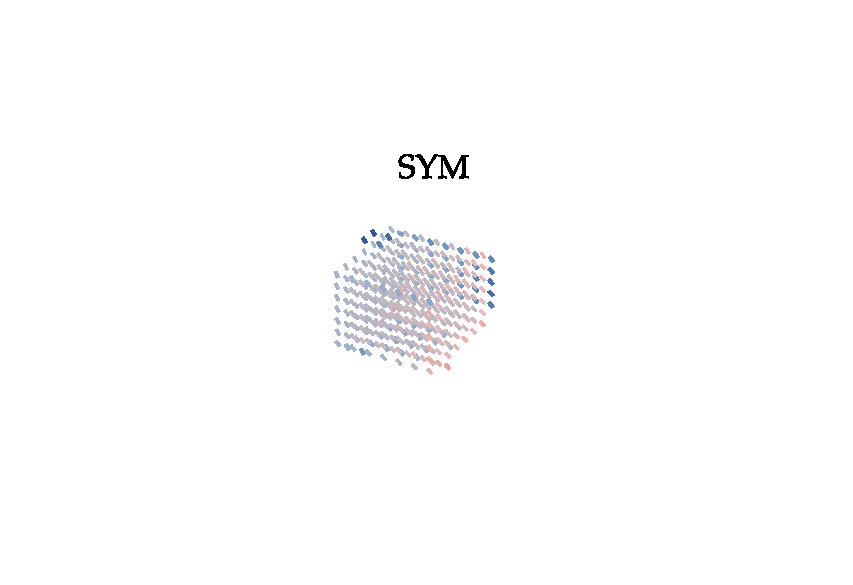
\includegraphics[trim={2.5cm 2.5cm 2.5cm 2.5cm},clip, width = 1\textwidth]{./svg-inkscape/P_3D_indSYM_svg-tex.pdf}
    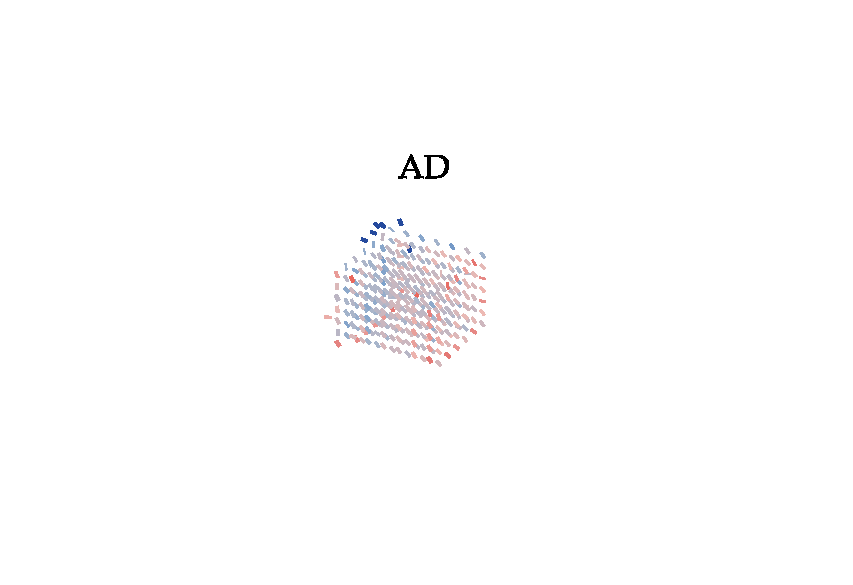
\includegraphics[trim={2.5cm 2.5cm 2.5cm 2.5cm},clip, width = 1\textwidth]{./svg-inkscape/P_3D_indAD_svg-tex.pdf}
    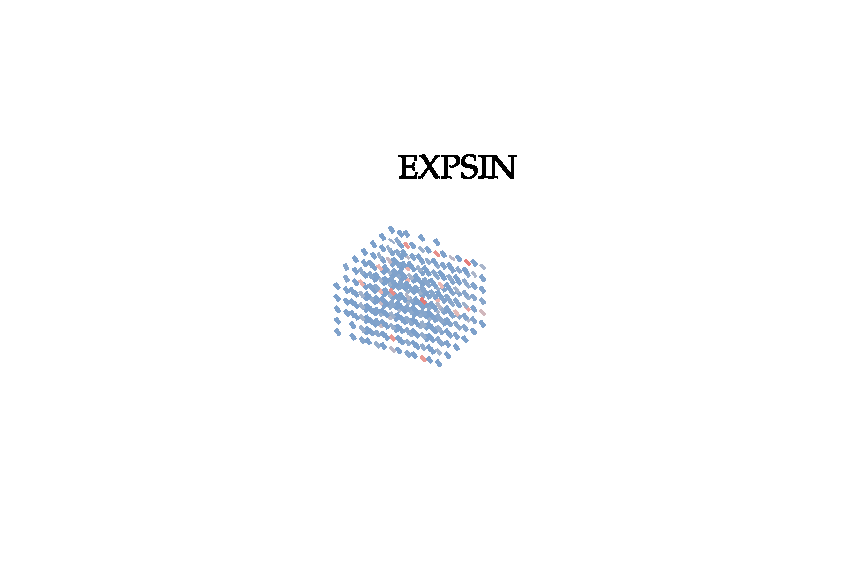
\includegraphics[trim={2.5cm 2.5cm 2.5cm 2.5cm},clip, width = 1\textwidth]{./svg-inkscape/P_3D_indEXPSIN_svg-tex.pdf}
    %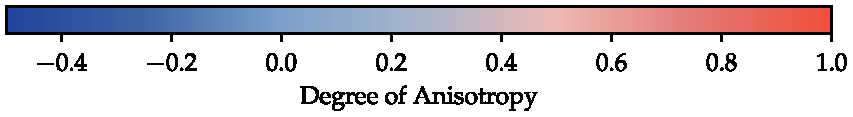
\includegraphics[width = 0.25\textwidth, right]{./svg-inkscape/P_3D_indcolorbar_svg-tex.pdf}
    \includesvg[]{../XRD_CT/Plotting/thesis_plots/P_3D_indcolorbar.svg}
    \caption[3D Reconstructions of Phantom Data Set]{ 3D reconstruction of the Phantom data set.
        The reconstruction has been cropped to the region of interest,
        and the degree of anisotropy has been plotted for voxels that have an isotropic intensity, meaning a0 or A, above a threshold of 0.1. }
    \label{fig:phantom_reconstruction_3D}
\end{figure}

\clearpage
A more in-depth analysis was performed on
the individual reconstruction parameters for the centremost 2D-slice, which are shown in Figure \ref{fig:phantom_reconstruction_2D} and \ref{fig:phantom_reconstruction_2D_angles}. % RSD: Describe
In regards to the isotropic intensity parameter, $a0$ or $A$, the different algorithms showed different degree of consistency.
Compared to the "AD"-algorithm, the "SYM"-algorithm had fewer and smaller outliers from the true value of isotropic intensity, which was 1.
However, the "SYM"-algorithm performed poorly at the interface between the sample and the surroundings.
Generally, the "EXPSIN"-algorithm's estimate of isotropic intensity was lower than the true value.
Apart from the low estimate, the "EXPSIN"-algorithm behaved similarly to the "AD"-algorithm.
Regarding the degree of anisotropy, the "SYM"-algorithm and the "AD"-algorithm showed similar behaviour.
The noise outside the edges of the sample was a result of the calculation of DoA where the intensity was zero.
Therefore, these artefacts can be neglected.
The "EXPSIN"-algorithm had no such noise, indicating that the anisotropy was not optimised properly.


%RSD: Also discuss anisotropy part, but wait for the proper metric. 

\begin{figure}[h!]
    \centering
    %RSD: For compilation:
    % \includesvg[]{../XRD_CT/Plotting/thesis_plots/P_slices_A.svg}
    % \includesvg[]{../XRD_CT/Plotting/thesis_plots/P_slices_DoA.svg}
    %RSD: Possible compilation issue if changing the plots
    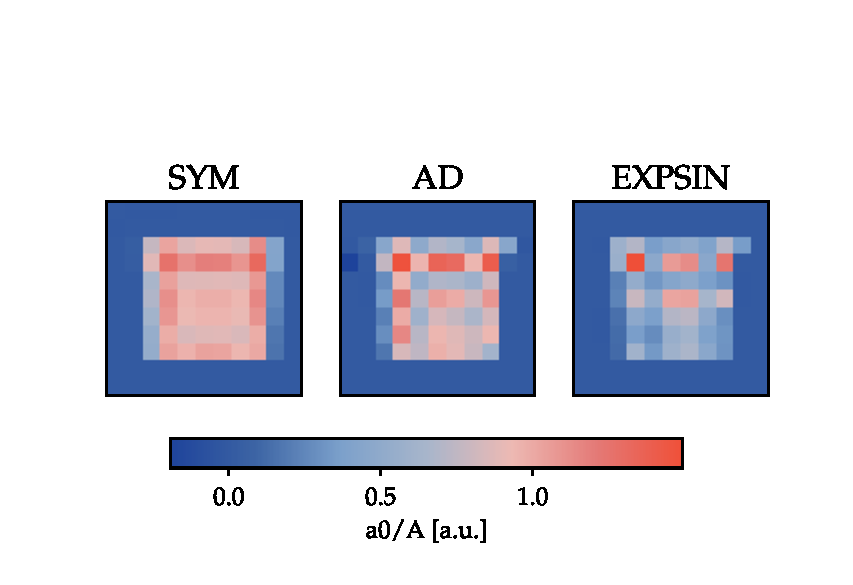
\includegraphics[trim={0 0cm 0 2.5cm},clip,width=1\textwidth]{./svg-inkscape/P_slices_A_svg-tex.pdf}
    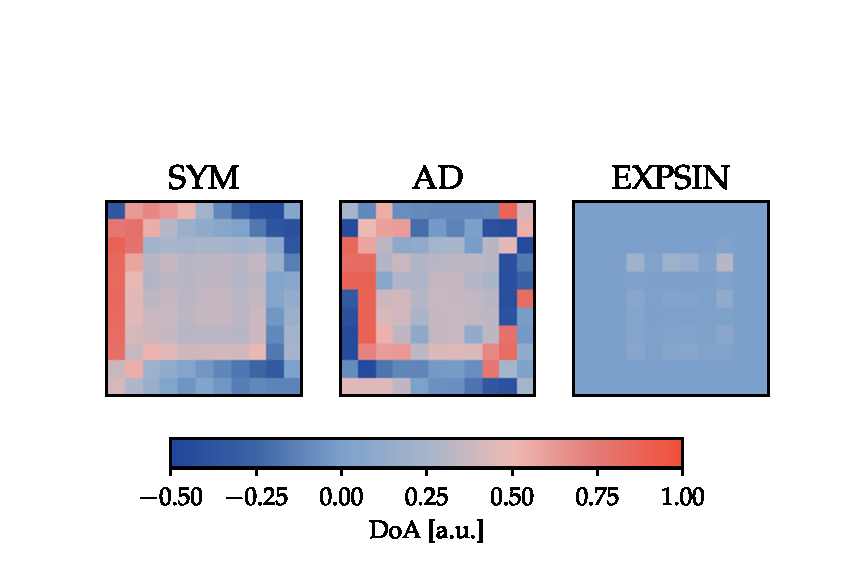
\includegraphics[trim={0 0cm 0 2.5cm},clip,width=1\textwidth]{./svg-inkscape/P_slices_DoA_svg-tex.pdf}
    %\adjustbox{trim = 0cm 1cm 0cm 0cm}{\includesvg[width = 1\textwidth]{../XRD_CT/Plotting/thesis_plots/P_slices_A.svg} }
    %\adjustbox{trim = 0cm 1cm 0cm 0cm}{\includesvg[width = 1\textwidth]{../XRD_CT/Plotting/thesis_plots/P_slices_B.svg} }
    %\adjustbox{trim = 0cm 0cm 0cm 3cm}{\includesvg[width = 1\textwidth]{../XRD_CT/Plotting/thesis_plots/P_slices_theta.svg}}
    %\adjustbox{trim = 0cm 0cm 0cm 3cm}{\includesvg[width = 1\textwidth]{../XRD_CT/Plotting/thesis_plots/P_slices_phi.svg}}
    \caption[Slice of Reconstructed Coefficients for Phantom Data Set]{ A 2D slice of the reconstructed volume that shows the isotropic parameter in the top figure, and the degree of anisotropy in the bottom figure, for the different reconstruction algorithms, respectively.
        More specifically, the slice where z = 17 is shown.}
    \label{fig:phantom_reconstruction_2D}
\end{figure}

\clearpage

Moreover, from Figure \ref{fig:phantom_reconstruction_2D_angles}, which shows the reconstructed preferred angles,
it is evident that the "EXPSIN"-algorithm had many voxels in the middle of the sample with the same set of preferred angles as the initial conditions.
In contrast, the same voxels had converged to the true angles in the "AD"-algorithm and the "SYM"-algorithm, respectively,
in terms of orientation.


\begin{figure}[h!]
    \centering
    %RSD: For compilation:
    % \includesvg[]{../XRD_CT/Plotting/thesis_plots/P_slices_theta.svg}
    % \includesvg[]{../XRD_CT/Plotting/thesis_plots/P_slices_phi.svg}
    %%%
    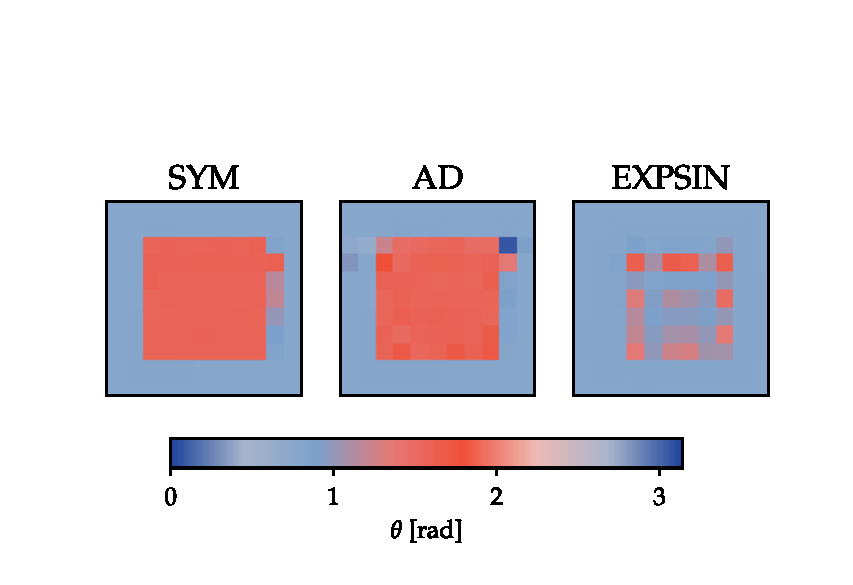
\includegraphics[trim = {0 0 0 2.5cm}, clip, width = 1\textwidth]{./svg-inkscape/P_slices_theta_svg-tex.pdf}
    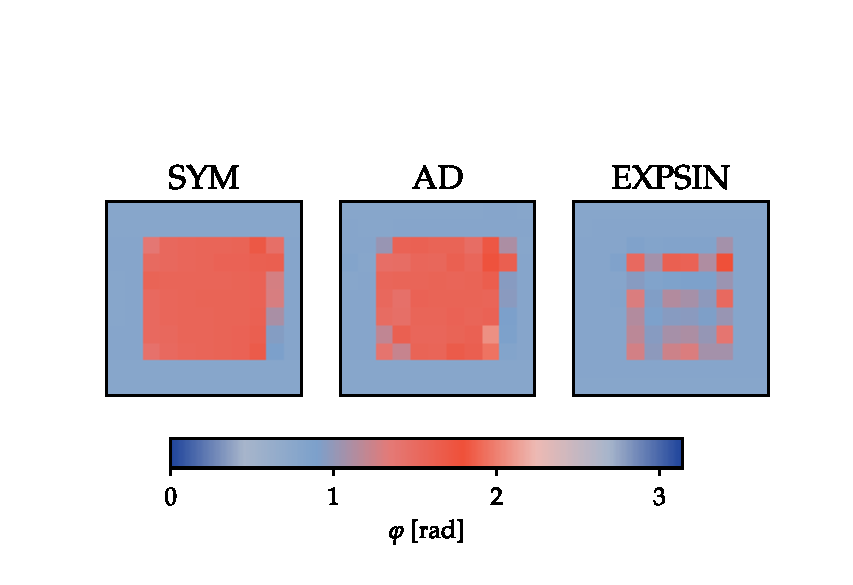
\includegraphics[trim = {0 0 0 2.5cm}, clip, width = 1\textwidth]{./svg-inkscape/P_slices_phi_svg-tex.pdf}
    \caption[Slice of Reconstructed Orientation for Phantom Data Set]{ A 2D slice of the reconstructed volume that shows the preferred orientation of the reconstructed nanostructures for the different reconstruction algorithms, respectively.
        The cross section where z = 17 is shown.}
    \label{fig:phantom_reconstruction_2D_angles}
\end{figure}




\clearpage
\section{Reconstruction of Physical Carbon Knot}\label{sec:reconstruction_physical_carbon_knot}

%The general reconstruction ability of the different gradient computation methods
As a final comparison of the different SAXSTT algorithms, the reconstruction of a physical carbon knot, using actual synchrotron data, was performed.
Figure \ref{fig:carbon_knot_reconstruction_3D} shows the 3D reconstruction of the carbon knot.
Again, the marker colour represents the degree of anisotropy, while the orientation of the nanostructures is represented by the direction of the markers.
% RSD: Describe Further
All the algorithms showed similar ability to segregate the voxels containing the carbon knot from the surrounding void.
However, the "EXPSIN"-algorithm had almost twice the number of voxels with an isotropic intensity above the threshold value of 6 compared to the other algorithms.
This is an indication of a blurred interface between the carbon knot and the surrounding void.
Nevertheless, the orientation parameters seem to be correctly estimated in all algorithms,
and all algorithms have captured the high degree of anisotropy, as expected in Section \ref{sec:data_set_carbon_knot}.
This observation is further verified in Figure \ref{fig:carbon_knot_ortho}, which shows different orthogonal projections of the reconstructed vector field.
Note that the colour bar has been shifted to contrast equatorial scattering intensities from isotropic scattering intensities,
as the amount of meridional scattering was proven to be negligible in Figure \ref{fig:carbon_knot_reconstruction_3D}.
The orientation of the nanostructures is represented by the direction of the markers
All voxels with an isotropic intensity below the threshold of 6 are not shown.

\clearpage

\begin{figure}[h!]
    \centering
    %RSD: For compilation:
    % \includesvg[width = 1\textwidth]{../XRD_CT/Plotting/thesis_plots/ck_indSYM.svg}
    % \includesvg[width = 1\textwidth]{../XRD_CT/Plotting/thesis_plots/ck_indAD.svg}
    % \includesvg[width = 1\textwidth]{../XRD_CT/Plotting/thesis_plots/ck_indEXPSIN.svg}

    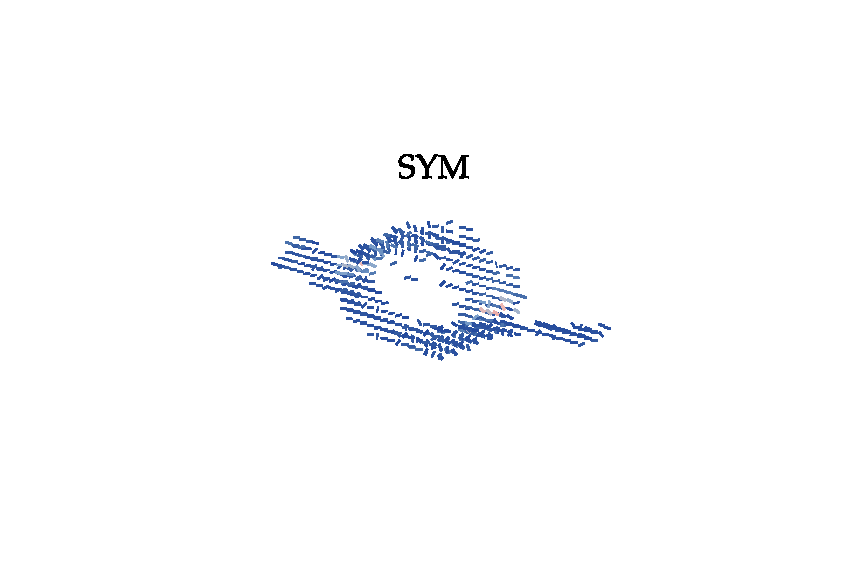
\includegraphics[trim={2.5cm 2.5cm 2.5cm 2.5cm},clip, width = 1\textwidth]{./svg-inkscape/ck_indSYM_svg-tex.pdf}
    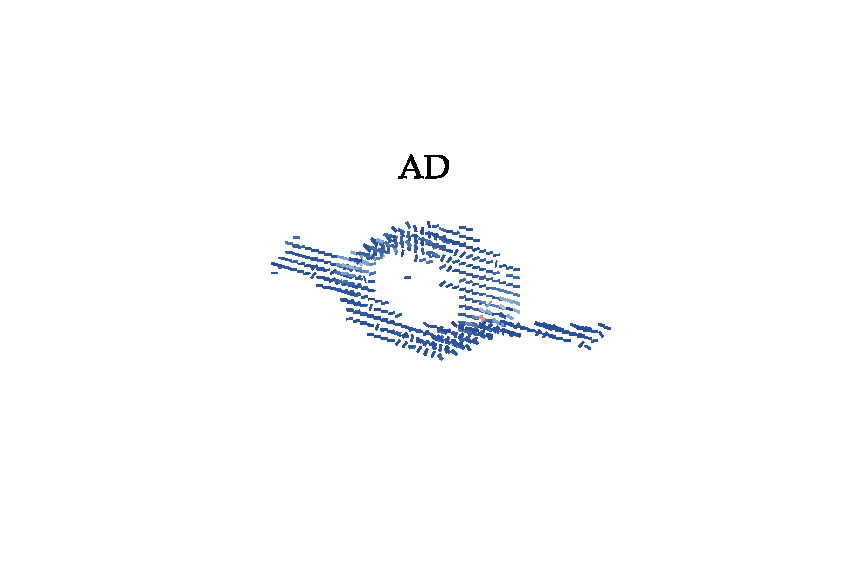
\includegraphics[trim={2.5cm 2.5cm 2.5cm 2.5cm},clip, width = 1\textwidth]{./svg-inkscape/ck_indAD_svg-tex.pdf}
    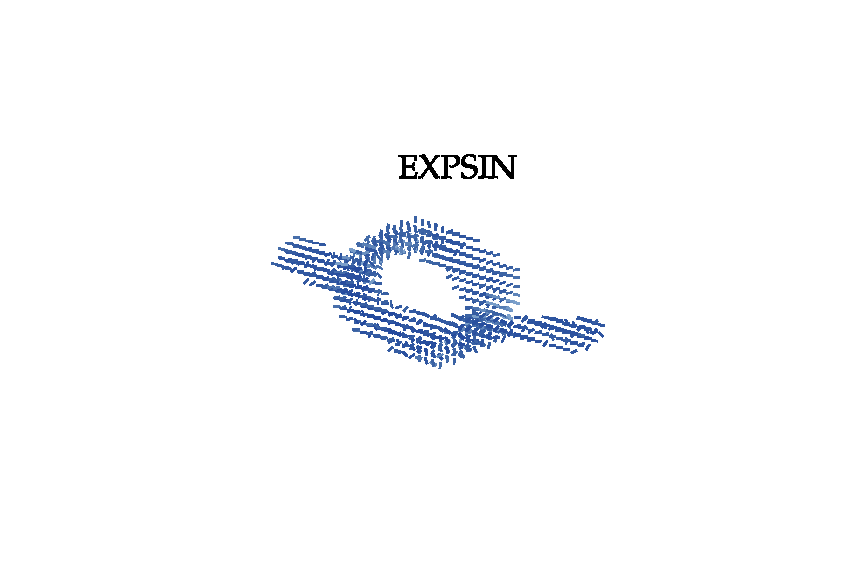
\includegraphics[trim={2.5cm 2.5cm 2.5cm 2.5cm},clip, width = 1\textwidth]{./svg-inkscape/ck_indEXPSIN_svg-tex.pdf}
    \includesvg[]{../XRD_CT/Plotting/thesis_plots/ck_indcolorbar.svg}

    \caption[3D Reconstructions of Carbon Knot]{ The resulting 3D reconstructions of the carbon knot from the "SYM"-, "AD"-, and "EXPSIN"-algorithm, respectively.
        There were 561, 533, and 900 voxels with an isotropic intensity above the threshold value of 6, respectively. Generally, the voxels point in the direction of the carbon fibers.
    }
    \label{fig:carbon_knot_reconstruction_3D}
\end{figure}

\clearpage

\begin{figure}

    \centering

    \includegraphics[width = \textwidth]{../XRD_CT/Plotting/thesis_plots/ortho_projections.pdf}
    \includesvg[width = 0.8\textwidth]{../XRD_CT/Plotting/thesis_plots/ortho_projectionscolorbar_equatorial.svg}
    \caption[Orthogonal Projections of Carbon Knot]{ Orthogonal projections of the carbon knot reconstructions.
        The rows of the figure show the respective reconstructions projected on the XY-, XZ-, and YZ-plane, respectively.
        Only voxels with an isotropic intensity above a designated threshold value of 6 are shown.
        Moreover, the included volume has also been cropped to only show most of the carbon knot.
        The colour of the markers are cold for equatorial anisotropy and warm for isotropic voxels, as indicated by the colourbar, while the orientation is represented by the direction of the markers.
    }
    \label{fig:carbon_knot_ortho}

\end{figure}

\clearpage

From the reconstructed volume, the centremost slice (z = 17) was investigated further.
Figure \ref{fig:carbon_knot_reconstruction_2D_coeffs} shows the isotropic coefficent, a0 or A, and the degree of anisotropy, DoA, reconstructed using symbolically, automatically, and alternatively calculated gradients, respectively.
Note that the a0 coefficient in some sense corresponds to coefficient A in the alternative cost function \eqref{eq:exp_sin_squared}, as both generally determine the scattering intensity from a voxel.
However, they are not quantitatively comparable.
%RSD: Describe. 
The results of the "SYM"- and "AD"-algorithm were close to indistinguishable,
while the "EXPSIN"-algorithm shared most of the same features.
However, the latter reconstruction had a less pronounced edge in terms of intensity at the interface between the sample and the surroundings.
In some sense it seems to be more of a rough estimate, and less converged than the two others.
With that being said, the amount of noise in surroundings of the DoA calculation was much less than for SYM and AD.

\begin{figure}[h!]
    \centering
    %RSD: For compilation:
    % \includesvg[width = 1\textwidth]{../XRD_CT/Plotting/thesis_plots/ck_slices_A.svg}
    % \includesvg[width = 1\textwidth]{../XRD_CT/Plotting/thesis_plots/ck_slices_DoA.svg}

    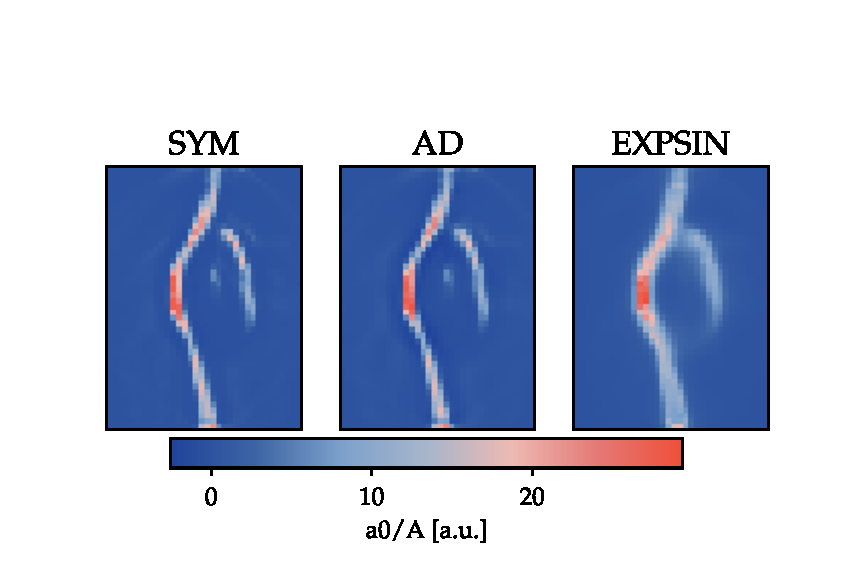
\includegraphics[trim = {0 0 0 2.0cm}, clip, width = 1\textwidth]{./svg-inkscape/ck_slices_A_svg-tex.pdf}
    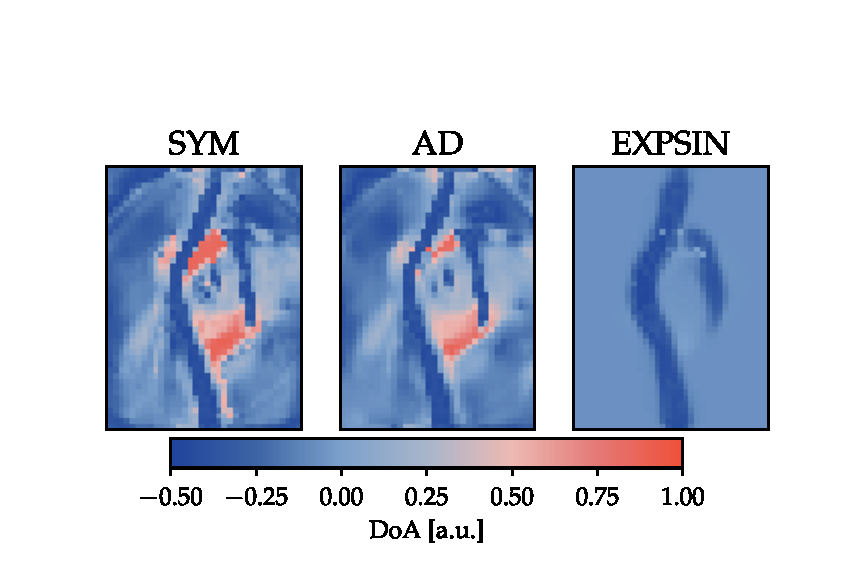
\includegraphics[trim = {0 0 0 2.0cm}, clip, width = 1\textwidth]{./svg-inkscape/ck_slices_DoA_svg-tex.pdf}

    \caption[Slice of Reconstructed Coefficients for Carbon Knot]{  A 2D slice of the reconstructed carbon knot that shows the isotropic parameter in the top figure, and the degree of anisotropy in the bottom figure, for the different reconstruction algorithms, respectively.
        More specifically, the slice where z = 17 is shown. }
    \label{fig:carbon_knot_reconstruction_2D_coeffs}
\end{figure}

\clearpage
The preferred orientations in the mentioned 2D slice are shown in Figure \ref{fig:carbon_knot_reconstruction_2D_angles}. %RSD: Describe
Again, the "EXPSIN"-result turned out to be noisy, even though the main features were reconstructed correctly.
It is interesting how a the main features are constructed correctly, but on a bigger scale, affecting more voxels, than the "SYM"- and "AD"-algorithms.
It is important to remember the only two differences between the implementations are the form factor in the cost function, and step-wise reconstruction versus all-at-once reconstruction.
In contrast to the isotropic and anisotropic parameters,
the "AD"-algorithm and the "SYM"-algorithm were slightly different in terms of preferred angles.
Nevertheless, the differences were small, and the edges between the sample and the surroundings were well-defined in both algorithms.

\begin{figure}[h!]
    \centering
    %RSD: For compilation:
    % \includesvg[width = 1\textwidth]{../XRD_CT/Plotting/thesis_plots/ck_slices_theta.svg}
    % \includesvg[width = 1\textwidth]{../XRD_CT/Plotting/thesis_plots/ck_slices_phi.svg}

    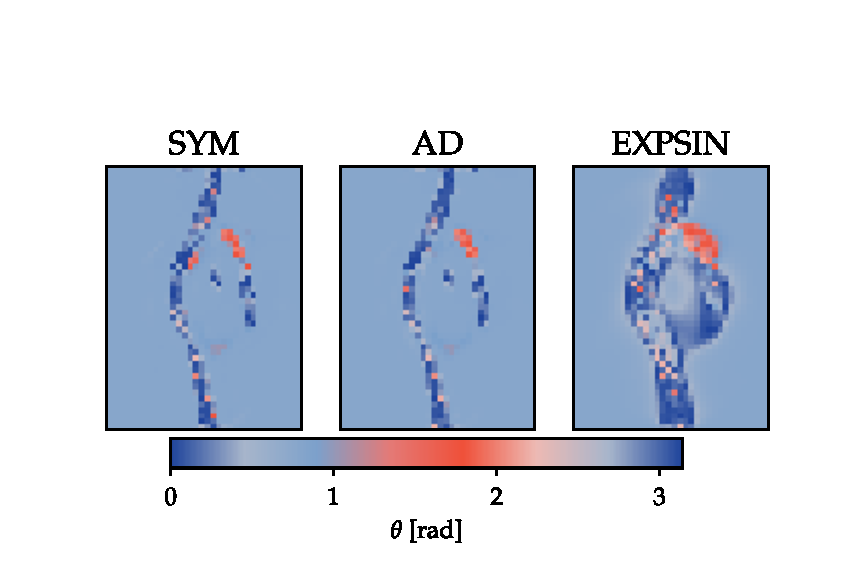
\includegraphics[trim = {0 0 0 2.0cm}, clip, width = 1\textwidth]{./svg-inkscape/ck_slices_theta_svg-tex.pdf}
    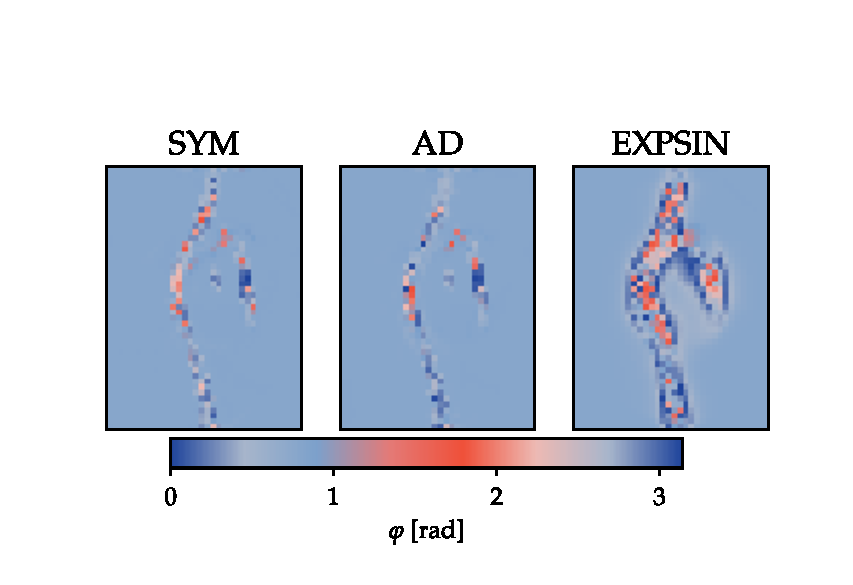
\includegraphics[trim = {0 0 0 2.0cm}, clip, width = 1\textwidth]{./svg-inkscape/ck_slices_phi_svg-tex.pdf}
    \caption[Slice of Reconstructed Orientation for Carbon Knot]{  The reconstructed preferred orientation of the carbon knot in the z=17 cross section for the different reconstruction algorithms, respectively.
        All the main features have been correctly reconstructed, but the "EXPSIN"-algorithm has a higher noise level where the features in some sense are magnified in extent. }
    \label{fig:carbon_knot_reconstruction_2D_angles}
\end{figure}




